\chapter{Appendix to Chapter~\ref{ch:icml}}

\section{Environment details}

This section provides additional details for the three types of inverse problem studied in our paper. All problems are implemented using the Pyro probabilistic programming framework~\cite{binghamPyroDeepUniversal2019}.

\subsection{Seismic Waveform Inversion}

An illustration of the SWI problem is given in Fig.~\ref{fig:swi_explainer}. We implement the SWI problem using the Deepwave library~\cite{richardsonDeepwave2023}. We use latent parameters $z \in \R^{n_x \times n_y}$ representing the subsurface density profile (with spatial resolution $n_x$ and $n_y$), context $y \in \R^{n_T}$ representing the source signal, and observations $x \in \R^{n_{s} \times n_{r} \times n_{T}}$ representing the signal measured at each receiver, where $n_s, n_r, n_T$ are the number of sources, receivers, and timesteps, respectively. The observations are corrupted with additive isotropic Gaussian noise.

\begin{figure}[ht]
    \centering
    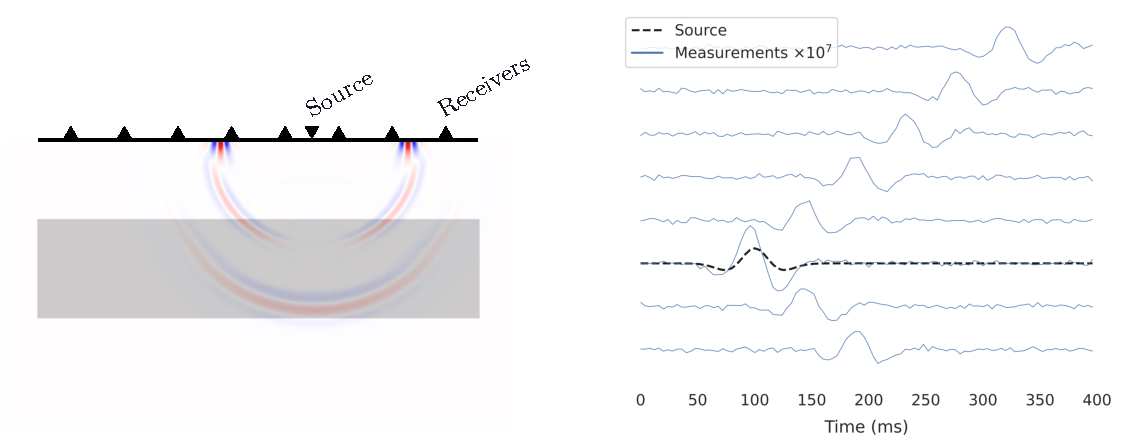
\includegraphics[width=0.6\linewidth]{figs/swi_results/swi_overview.pdf}
    \caption{(Left) An illustration of the SWI problem and (right) the receiver measurements (blue) given a source signal (black).}
    \label{fig:swi_explainer}
\end{figure}

\subsection{UAV Control}

We model the nonlinear attitude dynamics of the UAV as a combination of an unknown linear mapping from the current and desired states to angular rates, then a nonlinear mapping from angular rates to updated UAV orientation. The state $q = [\phi, \theta, \psi]$ includes the roll, pitch, and yaw angles of the UAV, and $\hat{q}$ denotes the commanded orientation. We model the angular rates of the UAV as
\begin{align}
    \omega = \mat{p \\ q \\ r} &= Aq + K (\hat{q} - q) + d + \eta
\end{align}
where $A$, $K$, and $d$ are unknown feedforward, feedback, and bias dynamics, and $\eta$ is Gaussian process noise. The state derivative is related to $\omega$ by
\begin{align}
    \der{}{t}q & = J^{-1}(q) \omega                                    \\
    J^{-1}(q)  & = \mat{
    1          & \tan(\theta)\sin(\phi)    & \tan(\phi)\cos(\theta)    \\
    0          & \cos(\phi)                & -\sin(\phi)               \\
    0          & \sin(\phi) / \cos(\theta) & \cos(\phi) / \cos(\theta)
    }
\end{align}

We apply a first-order time discretization to yield the one-step stochastic dynamics
\begin{align*}
    q_{t+1} & = q_t + \delta_t J^{-1}(q) \pn{Aq + K (\hat{q} - q) + d + \eta}
\end{align*}
and observed states are additionally corrupted by Gaussian noise.